\documentclass[12pt,a4paper]{scartcl}
\usepackage{tikz}
\begin{document}
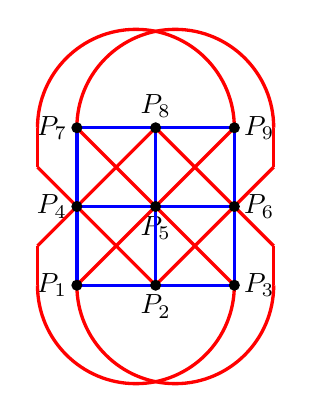
\begin{tikzpicture}
			\coordinate[label=left:$P_1$] (P1) at (0,0);
			\coordinate[label=below:$P_2$] (P2) at (1,0);
			\coordinate[label=right:$P_3$] (P3) at (2,0);
			\coordinate[label=left:$P_4$] (P4) at (0,1);
			\coordinate[label=below:$P_5$] (P5) at (1,1);
			\coordinate[label=right:$P_6$] (P6) at (2,1);
			\coordinate[label=left:$P_7$] (P7) at (0,2);
			\coordinate[label=above:$P_8$] (P8) at (1,2);
			\coordinate[label=right:$P_9$] (P9) at (2,2);

			% Horizontale blaue Geraden
			\draw[blue, very thick] (P1) -- (P3);
			\draw[blue, very thick] (P4) -- (P6);
			\draw[blue, very thick] (P7) -- (P9);
			
			% Vertikale blaue Geraden
			\draw[blue, very thick] (P1) -- (P7);
			\draw[blue, very thick] (P2) -- (P8);
			\draw[blue, very thick] (P3) -- (P9);
			
			% Rote Diagonalen		
			\draw[red, very thick] (P1) -- (P9);
			\draw[red, very thick] (P3) -- (P7);
			
			% Rote Halbkreise oben
			\draw[red, very thick] (P7) arc (180:0:1.25);
			\draw[red, very thick] (P9) arc (0:180:1.25);
			
			% Rote Geraden nach oben verbunden
			\draw[red, very thick] (P2) -- (2.5,1.5);
			\draw[red, very thick] (2.5,1.5) -- (2.5,2);
			\draw[red, very thick] (P2) -- (-0.5,1.5);
			\draw[red, very thick] (-0.5,1.5) -- (-0.5,2);
						
			% Rote Halbkreise oben
			\draw[red, very thick] (P1) arc (-180:0:1.25);
			\draw[red, very thick] (P3) arc (0:-180:1.25);				
			% Rote Geraden nach unten verbunden
			\draw[red, very thick] (P8) -- (2.5,0.5);
			\draw[red, very thick] (2.5,0.5) -- (2.5,0);
			\draw[red, very thick] (P8) -- (-0.5,0.5);
			\draw[red, very thick] (-0.5,0.5) -- (-0.5,0);
			
			% Punkte
			\fill (P1) circle (2pt);
			\fill (P2) circle (2pt);
			\fill (P3) circle (2pt);
			\fill (P4) circle (2pt);
			\fill (P5) circle (2pt);
			\fill (P6) circle (2pt);
			\fill (P7) circle (2pt);
			\fill (P8) circle (2pt);
			\fill (P9) circle (2pt);
			
			
		\end{tikzpicture}
